\documentclass[12pt]{article}

%\documentclass[fleqn]{article}
%\usepackage{palatino} 
%\usepackage{charter}
%\usepackage[T1]{fontenc}
%\usepackage{concmath} % pretty good
%\usepackage{cmbright}
%%%%%%%%%%%%%%%%%%%%%%%%%%%%%%%%%%%%%
\usepackage{/home/sci/weiliu/haldefs}
\usepackage{/home/sci/weiliu/notes}
\usepackage{/home/sci/weiliu/projects/lwdefs}
\usepackage{graphicx}
\usepackage{url}
\usepackage{textcomp}
%\usepackage[numbers]{natbib}
\usepackage{natbib}
\usepackage{subfig}
\usepackage{hyperref}
\usepackage{/home/sci/weiliu/packages/breakurl/breakurl}
%\usepackage{endfloat}
\usepackage{amsmath}
\usepackage{verbatim}
\usepackage{natbib}
\usepackage{algorithmic}
\usepackage{algorithm}

\hypersetup{
    bookmarks=true,         % show bookmarks bar?
    unicode=false,          % non-Latin characters in Acrobat’s bookmarks
    pdftoolbar=true,        % show Acrobat’s toolbar?
    pdfmenubar=true,        % show Acrobat’s menu?
    pdffitwindow=false,     % window fit to page when opened
    pdfstartview={FitH},    % fits the width of the page to the window
    pdftitle={Markov Random Field and fMRI},    % title
    pdfauthor={Author},     % author
    pdfsubject={Subject},   % subject of the document
    pdfcreator={Creator},   % creator of the document
    pdfproducer={Producer}, % producer of the document
    pdfkeywords={keywords}, % list of keywords
    pdfnewwindow=true,      % links in new window
    colorlinks= true,       % false: boxed links; true: colored links
    linkcolor=red,          % color of internal links
    citecolor=green,        % color of links to bibliography
    filecolor=magenta,      % color of file links
    urlcolor=cyan           % color of external links
}



\begin{document}
\title{Notes: Markov Random Fields and fMRI}
\author{Wei Liu}
\maketitle
\tableofcontents
%\newpage
\section{Ising Model}
In this section I did test on Ising model. Following example 1 in \cite{perez_markov_1998}, I sampled the prior the distribution of hidden variable $\vec x$ on a $255\times 255$ binary images. Results at fig. \ref{fig1}.

Also apply Ising prior on a image denoising application: 1) Get a original image and apply 10\% noise. 2) denoise with no spatial prior, with little and much prior. Results at fig. \ref{fig2}.

\begin{figure}[hbt]
\centering
\includegraphics[width = 0.24\textwidth]{figures/Ising1.eps} 
\includegraphics[width = 0.24\textwidth]{figures/Ising300.eps}
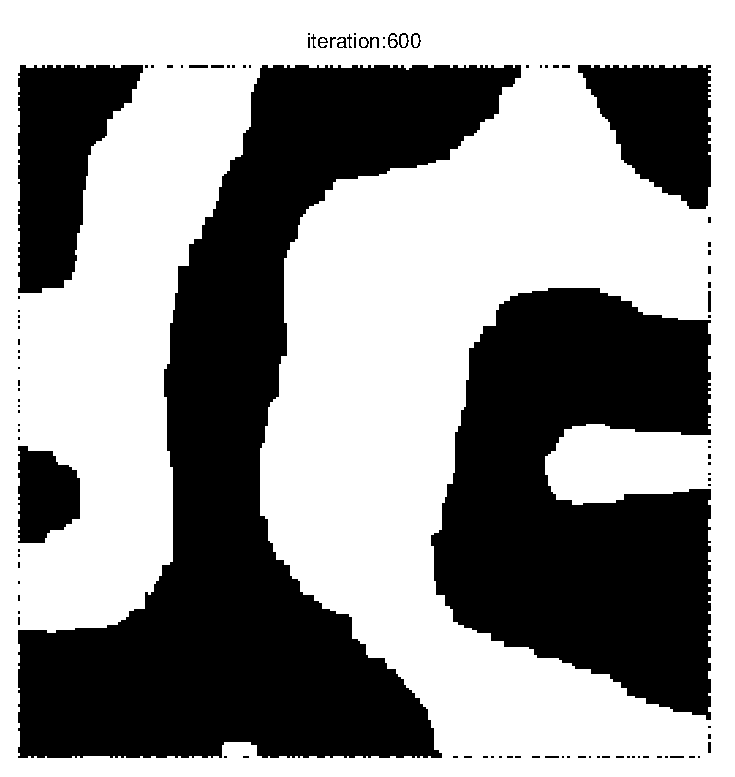
\includegraphics[width = 0.24\textwidth]{figures/Ising600.eps}
\includegraphics[width = 0.24\textwidth]{figures/Ising900.eps}

\caption{Initial image with uniform random -1 an +1. Update eqch pixel in sequence by the conditional probability. And repeat this many 1000 times. Here is the iteration for 1st time, 300, 600 and 900.}
\label{fig1}
\end{figure}

\begin{figure}[hbt]
\centering
\includegraphics[width = 0.8\textwidth]{MarryChristmas.eps}
\caption{$\beta$ controls how strong the prior is, compared to the conditional likelihood $P(\vec y |\vec x)$. Greater $\beta$ means the energy function prefer prior rather than data.}
\label{fig2}
\end{figure}
\subsection{Generate Ising model by Gibbs Sampling}
In this test I want to generate a Ising model using Gibbs sampling. The possible gray level for each data point is {-1, 1} and I'm going to use Gibbs sampling method to generate the prior image in Gibbs distribution.

The Gibbs distribution is defined by
\begin{equation}
P(\vec x) = \frac{1}{\mat Z}\exp\{-\mat U(x)\}
\end{equation}
The conditional probability of data point $x_s$ is given by
\begin{align}
p(x_s | x_{i\neq s}) &= \frac{\frac{1}{\mat Z}\exp\{-\sum_{C\in \mathcal{C}}V_C (\vec x_C)\}}{\sum_{x_s = 0}^{M-1}\frac{1}{\mat Z}\exp\{-\sum_{C\in \mathcal{C}}V_C (\vec x_C)\}} \\
 &= \frac{\frac{1}{\mat Z}\exp\{-\sum_{C:s\in C}V_C (\vec x_C)\}}{\sum_{x_s = 0}^{M-1}\frac{1}{\mat Z}\exp\{-\sum_{C: s\in C}V_C (\vec x_C)\}} \\
&= \frac{\exp\{-\sum_{C:s\in C}V_C (\vec x_C)\}}{\sum_{x_s = 0}^{M-1}\exp\{-\sum_{C: s\in C}V_C (\vec x_C)\}} \\
\end{align}

So we only need to compute the potential function for those $V_C$ that include $x_s$. Define $V_C$ as 
\begin{equation}
V_C(x_i, x_j) = \left \{
\begin{array}{l l}
1 \quad \mbox{when } x_i \neq x_j\\
0 \quad \mbox{when } x_i = x_j\\
\end{array} \right .
\end{equation}
We don not need to have bigger potential function value for those $|x_i - x_j|$ is large, because $x_i$ and $x_j$ as labeling, should make no difference on potential as long as they are different.

The difference between Gibbs sampling and Metroplis Sampling is, Gibbs sampling need to compute conditional probability of $p(x_s | x_{i\neq s})$, which take much computation when th possible value of $x_s$ is large. For binary image like Ising model, possible value of $x_s$ is just two, and Gibbs Sampling has no problem computing that.

\begin{figure}
\centering
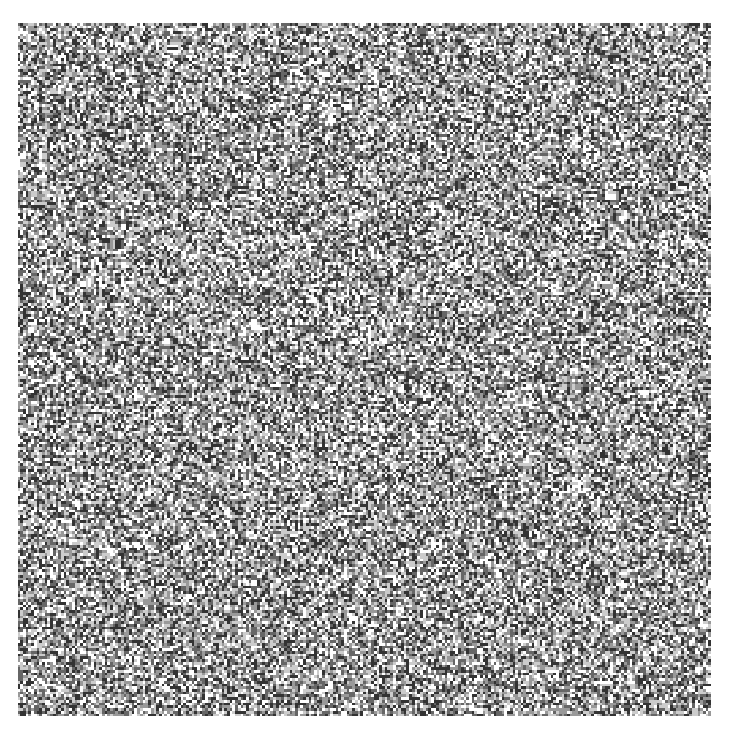
\includegraphics[width = 0.24\textwidth]{figures/Gibbs01.eps} 
\includegraphics[width = 0.24\textwidth]{figures/Gibbs200.eps} 
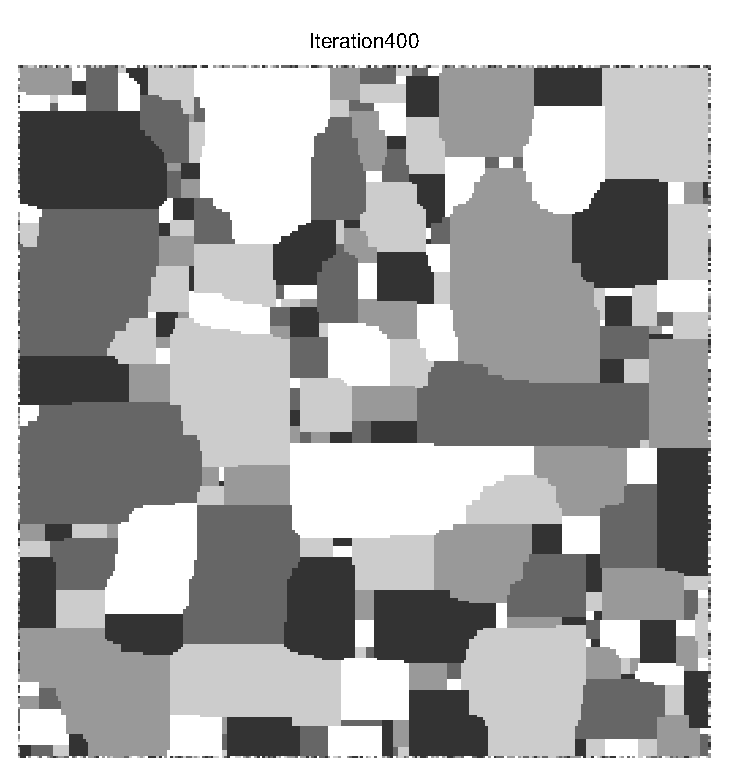
\includegraphics[width = 0.24\textwidth]{figures/Gibbs400.eps} 
\caption{Gibbs sampling to generate Gibbs distribution. Upper-left is the random generated  original 255x255 image with five gray level intensity. Upper-right is after 300 iterations of Gibbs sampling, with each iteration having raster scan through each pixel. Lower images are iterations 400 and 600 times.}
\label{Gibbs01}
\end{figure}

Figure \ref{Gibbs01} is the simulation result


Question: When the possible gray level is more than two, how do I generate them in Gibbs distribution (suppose I can compute the probability of each possible value, i.e. $P(\vec x = x_0)$, $P(\vec x = x_1)$, ... (Solved)
\subsection{Jan 19 Generate 1D fMRI image and compute posterior distribution}
\begin{figure}
\centering
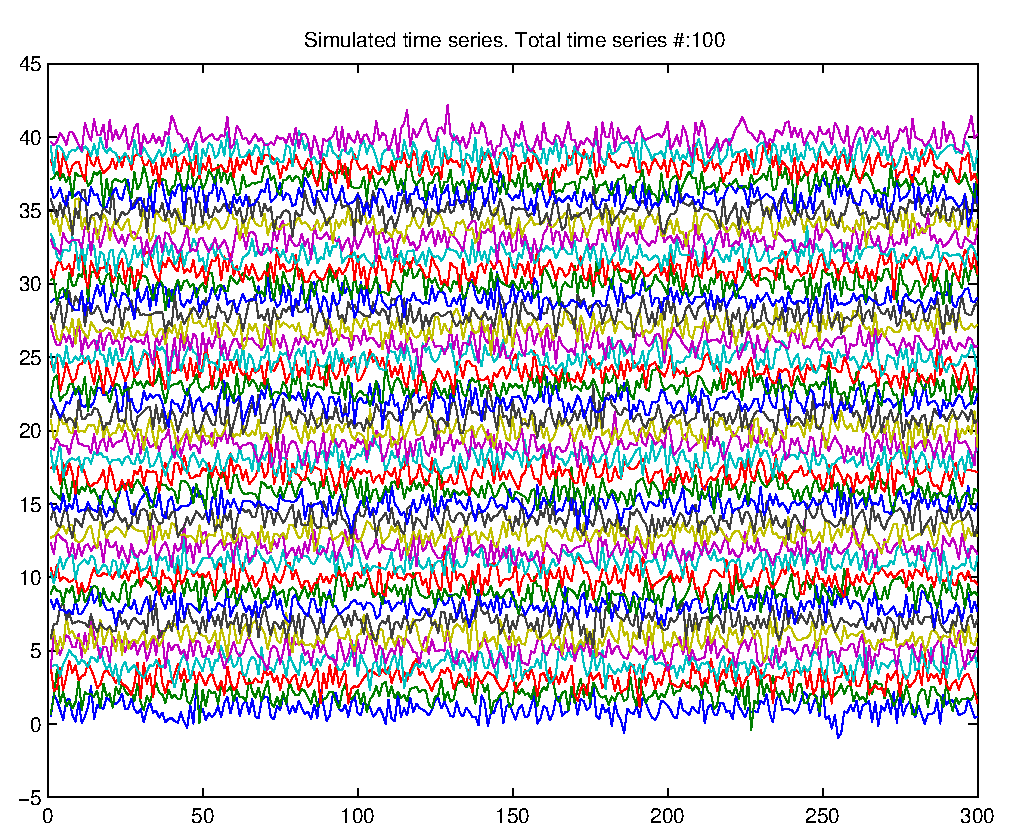
\includegraphics[width = 0.95\textwidth]{1DTimeSeries.eps} 
\caption{Generate N time series. Some are sin wave + Gaussian noise, others are purely Gaussian noise. Visualize them in a single plot by shifting the mean of each time series according to its label (from 1 to N)}
\label{1D}
\end{figure}

\begin{figure}
\centering
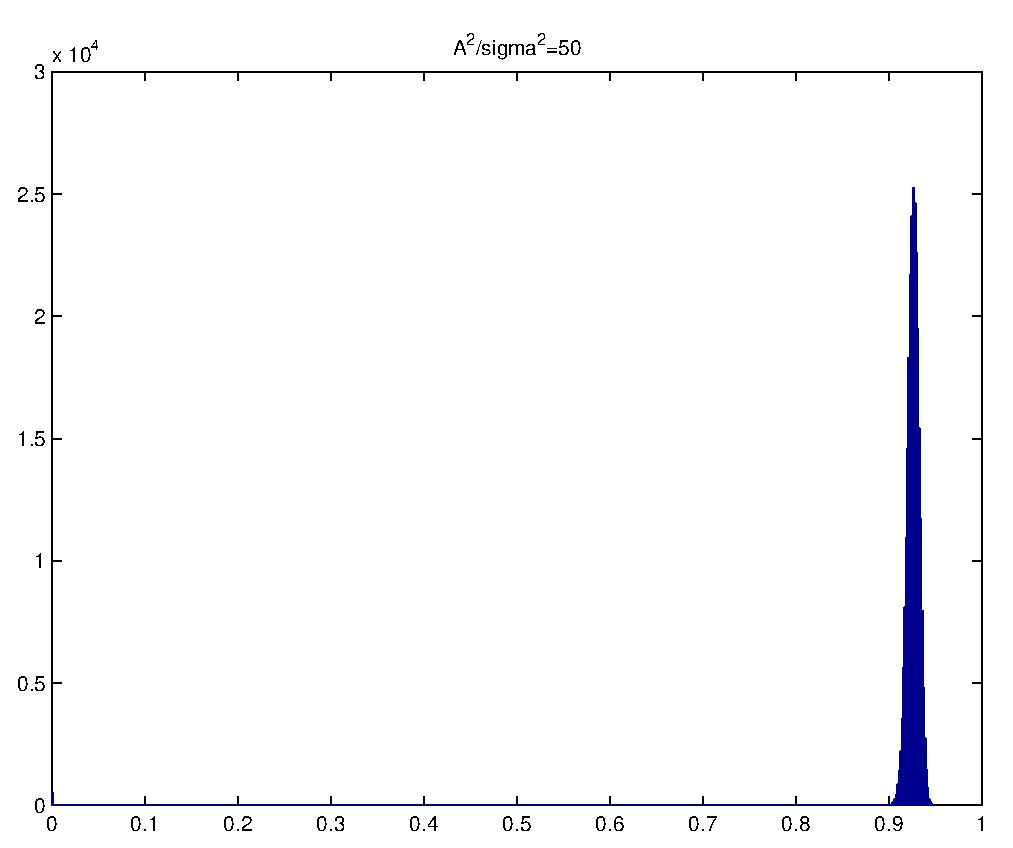
\includegraphics[width = 0.24\textwidth]{figures/empriLL50.eps} 
\includegraphics[width = 0.24\textwidth]{figures/empriLL20.eps} 
\includegraphics[width = 0.24\textwidth]{figures/empriLL10.eps} 
\includegraphics[width = 0.24\textwidth]{figures/empriLL2.eps} \\
\includegraphics[width = 0.24\textwidth]{figures/empriLL50z.eps} 
\includegraphics[width = 0.24\textwidth]{figures/empriLL20z.eps} 
\includegraphics[width = 0.24\textwidth]{figures/empriLL10z.eps} 
\includegraphics[width = 0.24\textwidth]{figures/empriLL2z.eps} 
\caption{The empirical distribution of the correlation between pair of $x_i$ and $x_j$ given they are 'connected'. To make them connected I generate all x from same sin wave plus independent Gaussian noise with different variance. A is amplitude of sin wave, and $\sigma$ is standard deviation of the Gaussian noise. I define $A^2/\sigma^2$ as the signal-to-noise ratio. On the bottom row is the empirical distribution of the z after Fisher Transformation. From Wikipeidia, Fisher transformation z is approximately normal only when 1) $x_i$ and $x_j$ are normal distribution, and 2) $x_i$ and $x_j$ are independent. Both conditions are not true in our case. But I just do the transformation and see the z's distribution.}
\label{1D}
\end{figure}

Two questions about Fisher transformation: 1) When data point $x$ and $y$ are not independent, is $z = 0.5*\ln (\rho+1/\rho-1)$ still approximately Gaussian distribution? 2) No matter if data point $x$ and $y$ are independent, to assume $z$ is approximately Gaussian, we must make sure sample correlation $r_i$ are independent over all $i = 1,...,N$. But in MRF, connectivity $c_i$is not independent, i.e. $P(c_i|c_{j\neq i} \neq p(c_i)$. Does this mean the p(r|c) is not independent?

I think even $c$ is not independent, $r_i$ is still independent given $c_i$, by the theory of conditional independence. That is, $p(r_1, r_2| c_1, c_2) = p(r_1|c_1)\cdot p(r_2|c_2)$. 

Now to compute posterior probability of connectivity $c$, I can use Gibbs Sampling(or Simulated Annealing) and EM algorithm to iteratively compute the posterior probability and model parameter. Here is the notations:
\begin{itemize}
\item $S$ is the set of lattice points.
\item $s$ is a lattice point, $s \in S $.
\item $X_s$ is the value of X at s. In our case, $X_s$ is the connectivity between two voxels. $X_s \in \{-1, 1\}$. It is also the latent variable we're interested in.
\item $\partial s$ is neighboring points of $s$.
\item $x_c$ is the value of $X$ at the points in clique $c$.
\item $V_c(x_c)$ is potential function.
\item $Y_s$ is correlation at site $s$. $y_s$ is sample correlation between two voxels. 
%\item $p(c)$ is prior distribution. By MRF theory, $p(c)$ is Gibbs distribution.
%\item $\rho$ is population correlation. 
%\item $r$ is sample correlation, as an estimation of $\rho$.
%\item $p(r|c)$ is likelihood function. In term of MRF, it is emission function.
%\item $p(c|r)$ is posterior function, the one we're interested. 
\end{itemize}

We do not know the likelihood. There are two options: 1) Assume a data model used to generate $Y$. For example, we can assume two data point $\tilde d_i$ and $\tilde d_j$ and assume they are clear signal without any noise. Further assume they are perfectly correlated. Then generate two noised signal $d_i = \tilde d_i + N_i$ and $d_j = \tilde d_j + N_j$. $N_i$ and $N_j$ are additive Gaussian noise term with zero mean. Then we try to compute probability $corr(d_i, d_j)$ given the fact $\tilde d_i$ and $\tilde d_j$ are perfectly correlated. 2) We can generate some sample correlation $y_s$ from data points $d_i$ and $d_j$ given $\tilde d_i$ and $\tilde d_j$ have correlation one. This can be see as Monte Carlo method. From figure \ref{1D} we see even $d_i$ and $d_j$ are correlated, their sample correlations are approximately Gaussian distribution after Fisher Transformation.

So I assume the likelihood function $p(y_s|x_s = 1)$ is Gaussian with unknown $\mu_1$ and $\sigma_1^2$. We already know $p(y_s|x_s=0)$ is Gaussian with know $\mu_0 = 0$. To compute both the posterior $p(X|Y)$ and the parameters $\mu_1$ and $\sigma_1^2$ and $\sigma_0^2$ try to use EM algorithm as below:
\begin{algorithm}                 
\caption{EM-Annealing}         
\label{alg1}                   
\begin{algorithmic}            
\REQUIRE Sample correlation matrix $\mat Y$ with $y_s$ the sample correlation between voxel $i$ and $j$.
%\ENSURE $y = x^n$
\STATE Init posterior matrix $\mat X: x_s = \argmax \ln p(Y_s | x_s; \theta) $.

\WHILE{Some Condition}
\STATE \textbf{E step: }

(1) Based on the current parameters $\vec \theta = \{\mu_0, \mu_1, \sigma_0^2, \sigma_1^2, \beta\}$, compute the posterior probability as
\begin{equation}
p(X_s | Y_s = y_s) = \frac{p(X_s)\cdot p(Y_s = y_s | X_s, \vec \theta)}{p(Y_s = y_s | \vec \theta)} \label{eq1z}
\end{equation}
(2) Repeatedly Do Gibbs Sampling from \eqref{eq1z} until the field stabilize.

(3) Based on current value of $X_s$, iteratively compute the mean field
\begin{align}
p(X_s | < X_{\partial s}>) &= \frac{1}{Z_s} \exp\{-\beta U_s(X_s | <X_{\partial s}>\}\\
Z_s &= \sum_{X_s\in \{-1, 1\}}^{}\exp\{-\beta U_s(X_s | <X_{\partial s}>\}\\
<X_s> &= \sum_{X_s\in \{-1, 1\}}^{} X_s \cdot p(X_s | <X_{\partial s}>)
\end{align}
\STATE \textbf{M step: }

(4) With compute data $\{X, Y\}$, estimate $\beta$ by maximizing log-likelihood of posterior probability of $X$. Because likelihood $p(Y | X)$ does not depend on $\beta$, we only maximize prior $p(X)$, which is Gibbs distribution. We use Newton's method. (To be added)

(5) Estimate $\mu$ and $\sigma^2$ by maximizing conditional log-likelihood $p(Y | <X>)$. (To be added)
\ENDWHILE
\end{algorithmic}
\end{algorithm}

\textbf{Issue 1: }If there is negative correlation in the sample correlation, we need to model this component. We need to look at the histogram of sample correlation on real data, and see if there is much negative correlation. If there is, we need to add another state for connectivity, i.e. $c_{ij} = -1$ to model this component.

\textbf{Issue 2: }Need to assume the latent variable 'connectivity' is continuous in $[0, 1]$, instead of the discrete $\{0, +1\}$ for current model. 

\textbf{Issue 3: } How to change the temperature $T$ in annealing of E step? Two option 1) Keep $T$ unchanged in each iteration of EM. That is, $T$ is constant over the annealing. Over all E step, T decreases.  2) $T$ decrease over annealing in a single E step of EM. At the beginning of annealing of each E step, $T$ begins with a high value. 

\textbf{Issue 4: } In terms of `neighbors', we can define two types of neighbors: `local neighbors' and `remote neighbors'. Local neighbors is those data points spatially close to the data we're interested in. Remote neighbors are data that are not necessarily spatially close, but are close according to some defined features (like DTI connection). And we can use Suyash's theory: to know current pixel, we not only look at its local neighbors (like MRF), and also look at its remote neighbors.

\textbf{issue 5: } When applying prior, we have to be careful not to smooth `edges'. When we find edges, we should not assume the pixels on two sides of edges are neighbors (either local neighbors, or remote neighbors). the edges are not given, but to be computed in the iteration algorithm. (need to study this later)

\textbf{Issue 5:} If we can assume the posterior distribution is also a Gibbs distribution,  we can use annealing on posterior Gibbs, instead of only on prior. In this method, there is an additional parameter $\alpha$ to control the weights between the prior energy and likelihood energy (update: From Gelman's paper, seems there is no such $\alpha$, posterior energy just sum of prior and likelihood energy, not weighted sum.)

To prove the posterior distribution $p(c_n | r_n)$ is also Gibbs distribution, we just need to prove it is Markov Random Field. Assume $\partial c$ is the neighbors of $c_n$, and $\tilde C$ is the set of other nodes that does not include $c_n$ and $\partial c$. We need to prove 
\begin{align}
p(c_n | r_n, \partial c, \tilde C) &= p(c_n | r_n, \partial c)
\end{align}
while we know that 
\begin{align}
p(c) &\sim \mbox{Gibbs}, \qquad  p(c_n|\partial c_n, \tilde C) = p(c_n | \partial c_n)\\
p(r_n | c_n ) &= \cN(\mu, \sigma^2) \\
\end{align}

Now rewrite the posterior as
\begin{align}
p(c_n | r_n, \partial c_n, \tilde C) &= \frac{p(c_n) \cdot p(r_n, \partial c_n, \tilde C | c_n)}{p(r_n, \partial c, \tilde C)} \\
&= \frac{p(c_n) \cdot p(r_n \ c_n) \cdot p(\partial c_n, \tilde C| c_n)}{p(r_n) \cdot p(\partial c_n, \tilde C)}\\
&= \frac{p(r_n | c_n)}{p(r_n)}\cdot p(c_n | \partial c_n, \tilde C)\\
&= \frac{p(r_n | c_n)}{p(r_n)}\cdot p(c_n | \partial c_n) \label{eq1}
\end{align}

\begin{align}
p(c_n | \partial c_n) &= \frac{p(c_n) p(r_n, \partial c_n| c_n)}{p(r_n, \partial c_n)}\\
&= \frac{p(c_n) \cdot p(\partial c_n| c_n) \cdot p(r_n | c_n)}{p(r_n) \cdot p(\partial c_n)}\\
&= \frac{p(c_n, \partial c_n) \cdot p(r_n | c_n)}{p(r_n) \cdot p(\partial c_n)} \label{eq2}
\end{align}

We see \eqref{eq1} and \eqref{eq2} are equal, so we prove the posterior is also Gibbs.

\textbf{SNR of functional MRI data: } It is better to view fMRI data as time series and define signal-to-noise ratio from signal processing standpoint, i.e. 
\begin{equation*}
SNR = \frac{P_{sig}}{P_{no}} = \(\frac{A_{sig}}{A_{No}}\)^2
\end{equation*}

According to this definition, the 'auditory' data set has SNR closet to 1.0. This is better than $SNR = A_{sig}/ \sigma_{no}^2$. If $SNR = A_{sig}/ \sigma_{no}^2 = 1$, we have at least one time point among 100 time point that can reach $3\sigma = 3$, and by signal processing definition, the SNR would be 1/3.



\bibliographystyle{plainnat}
\bibliography{/home/sci/weiliu/projects/zotero}
\end{document}
